%!TEX root = ../thesis.tex
%*******************************************************************************
%*********************************** First Chapter *****************************
%*******************************************************************************
\renewcommand{\baselinestretch}{1.5}

\begin{chapter}{Introduction}

\section{General objetive and motivations}

Particle physics is a field of study of physics that studies the particles that create matter and its interactions to very small scale, even smaller than atoms. The particles analized in particle physics are the fundamental particles that compose the matter and the responsibles for all forces of nature. All thoses particles  and their properties are grouped in a theory called the Standard Model. Standard Model (SM) is a theory that describes the fundamental forces (except gravity) and classify the elementary particles in bosons (entire spin) and fermions (half spin).
The SM , created almost 50 years ago, has been the most successul theory in explain the phenomena in the subatomic world.
\\

One of the particles of the SM, the Higgs Boson , was recently discovered in 2012 in the ATLAS and CMS experiments at CERN. The discovery of Higgs boson in  proton proton collisions  marked a new era in the particle physics due to its characteristic  of giving the matter the property of mass, according to previous theories and predictions . Since then, people around the world are working in the Large Hadron Collider at CERN  in order to detect the Higgs bosons in higher energies and differents Higgs production processes. 
Also the impact of Higgs is also  important in cosmology,  where theoretical investigations relate the Higgs boson and the cosmic inflation.\\

In the recent years, there have been many studies in the Higgs production processes at CERN in pp collisions , such as gluon fusion (ggF), VBF, WH, ZH and $t\bar{t}$H and people have obtained consistent results in the search of Higgs in those processes. 
In this work, we will analize the production of Higgs boson in association with a
single top quark (tH) in proton-proton collisions with the CMS experiment of the LHC. 
The motivation of the work is this mechanism of production of the Higgs boson has not been observed before by any experiment. The exploration of Higgs production on the tH channel is subject relatively new. %The SM is used to study the tH channel and compare it with other Higgs production mechanisms results.
\\
Many channels are yet out of
reach experimentally. At the same time, many theoretical
proposals are yet to be put on test. It is possible that studies on the Higgs boson give evidence of small deviations from the SM  and test new physics that are beyond SM such as String Theory and  Supersymmetry. \\
%********************************** % Third Section  *************************************


\section{The Standard Model}  %Section - 1.3 
The SM, created in the decade of seventies, is a successful theory that explains the structure of matter and the interactions of three of the four fundamental forces which are electromagnetic, strong and weak forces. The gravitational force is yet to be included due to the scale of interaction with respect to the other 3.  All the matter is composed of three kinds of particles: leptons, quarks and bosons, also called mediators.\\

For the leptons we have electrons ($e$), muons ($\mu$), and taus ($\tau$) with charge -1 and their neutrinos $\nu_e, \nu_\mu,\nu_\tau$, are chargeless particles. Leptons have their respective antiparticle; same structure with opposite charge. 
 All of them have a spin (intrinsic angular momentum) of $\frac{1}{2}$\cite{griff}.% In case of neutrinos, so far experimentalists have found these have very small masses, but in the theoretical scheme, they are massless. \\
\\

 Quarks combine to form composite particles called hadrons. Quarks cannot be found in isolation, they always exist in form of hadrons that can be mesons or baryons. \\
Mesons , are bosons made up of a quark-antiquark pair, such as pion ($\pi$) and kaon ($K$).Mesons were theorized by Yukawa in 1937 and discovered in 1947 by Powell\cite{griff}.
Baryons are fermions made of 3 quarks. Examples of baryons are protons and neutrons. Both particles can interact via strong force.
\\

Quarks were first theorized by Murray Gell-Mann and 
George Zweig in 1964, were introduced as parts of an ordering scheme for hadrons, and there was little evidence for their physical existence until scattering experiments at the Stanford Linear Accelerator Center in 1968\cite{griff}.
There are 6 of them: up (1968), down (1968), strange (1968), charm (theorized in 1970, discovered 1974), bottom (theorized 1973, discovered 1977), top (theorized 1973, discovered 1995).
\\

Quarks have characteristics such as  electric charge, mass, color charge, and spin. The quarks up, charm and top have in common a charge of $\frac{2}{3}$, while the down , strange and bottom quarks have charge of $-\frac{1}{3}$. Among them , the top quark is the most massive of all, while the up and down are the least massive. 
The lepton and quarks have their respective antiparticle, which have the same mass, but inverted charge.\\  
Some of the particles in the SM are not stable, so they decays and form particles with lower masses. Other particles do not decay or their lifetimes are very long. The final states can be represented with a Feynman diagram according to the SM vertices\cite{mark}.

\begin{center}
    \begin{figure}[!htbp]
        \centering
        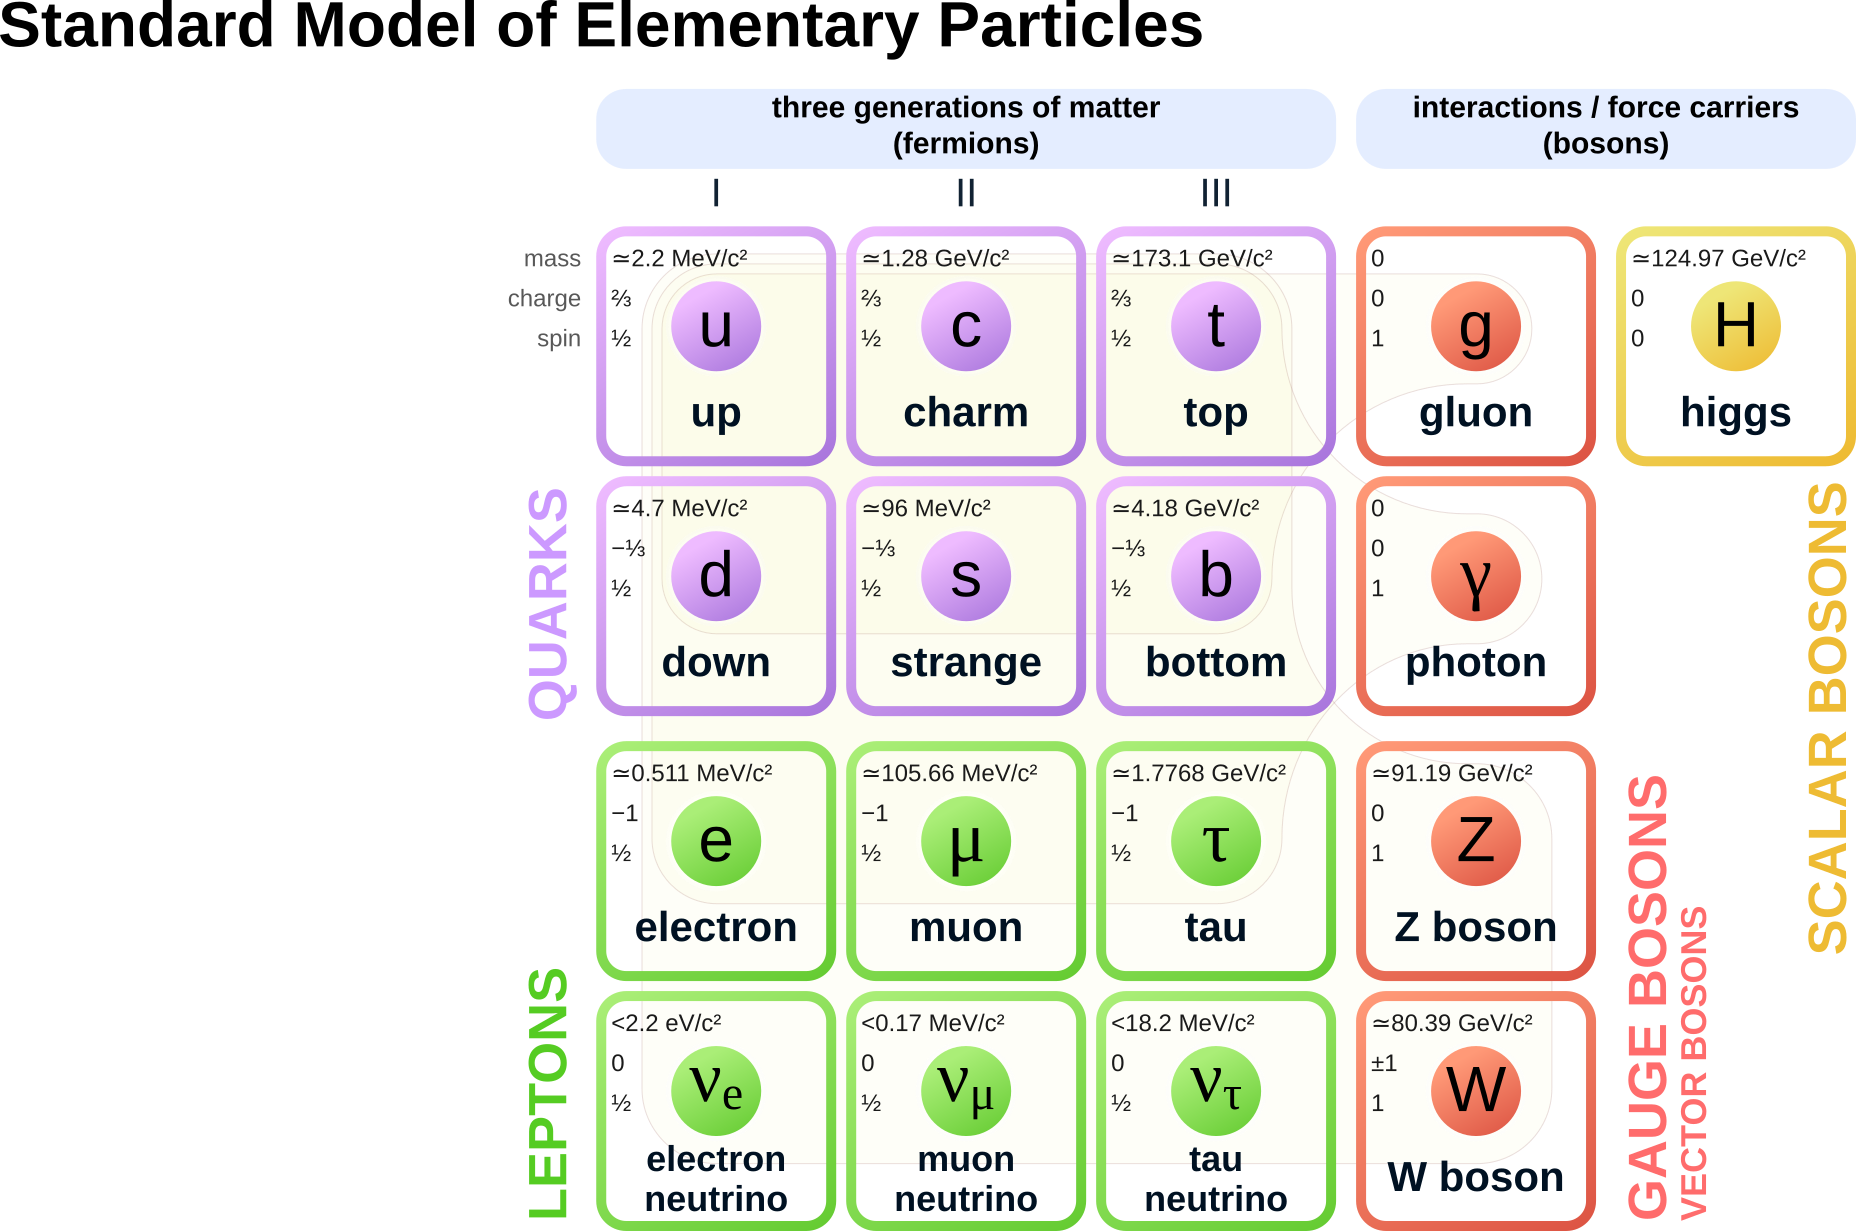
\includegraphics[scale=0.3]{Chapter1/sm1.png}
        \caption{Standard Model to date \protect \footnotemark}
        \label{sm1}
    \end{figure}
\end{center}
 \footnotetext{Taken from \url{https://upload.wikimedia.org/wikipedia/commons/0/00/Standard_Model_of_Elementary_Particles.svg}
} 

The last group of the family are the bosons,which have a spin 1 and 0. 
There are 5 bosons: $W^{\pm}$ , $Z$ with neutral charge are responsibles for weak force; photon, a massless particle, is responsible for electromagnetic force; gluon which also massless, is related to strong force and Higgs boson, recently discovered , is in charge of give the property of mass to particles via Higgs mechanism. Bosons let other particles to interact, even themselves, which is shown in the figure \ref{sm}. 
\\
The $W$,$Z$  and Higgs bosons, can interact with the most of the particles, while the gluon can only interact with quarks and itself.
Those bosons act as mediators in decays and creation of complex
particles, as mesons and baryons.\\

%In case of gravity, exist a theoretical particle, called graviton, that is the fundamental particle associated with the gravitational force. In case of its existance, it should have a spin 2 and mass 0. 

\begin{center}
    \begin{figure}[!htbp]
        \centering
        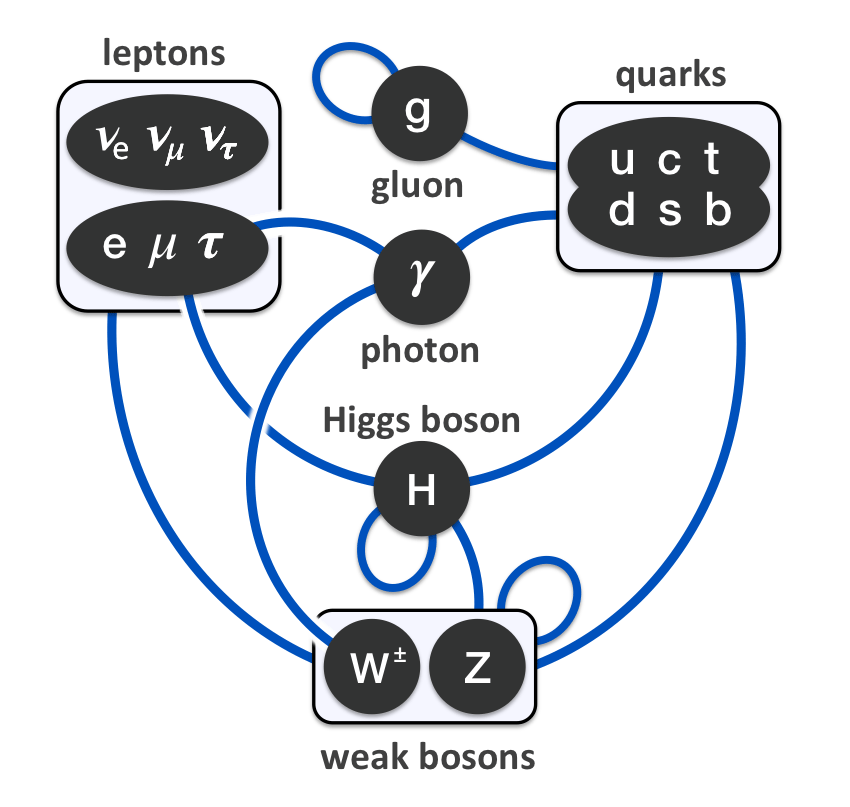
\includegraphics[scale=0.35]{Chapter1/sm.png}
        \caption{Particle interactions in Standard model}
        \label{sm}
    \end{figure}
\end{center}

There are experiments that detects particles around the world, such as the large hadron collider (LHC) in Europe, the Fermilab  in United States of America, KEK in Japan, etc. More information about the LHC will be described in the next chapters.
\\
Since quarks and gluons only exist in bound states, it is imposible to observe isolated quarks except the top quark, which decays before it has time to form a
bound state. As two quarks are separated, the strong force between them increases
which is equivalent to the potential energy increasing. This energy transforms into
quark-anti-quark pairs. \\

The table \ref{SM table} contains the characteristics of each particle in the SM. Note the distance column refers to particles moving with speeds near light speed. This column visualize the distance traveled in the predicted lifetime of the particle. And also give us a perspective of how hard is the detection of the particles due to lifetime. Stable lifetime means that the particles do not decay or can exist until they can interact with detectors. \\

\begin{table}[!htbp]
\caption{Table of particles in SM\cite{pd}. Stable means no decay, or lifetime almost infinite. Particles speeds at 0.998c}
\renewcommand{\arraystretch}{1.5}
\begin{tabular}{|c|c|c|c|c|p{2.5cm}|}
\hline 
Particle	& Mass (MeV/$c^2$)  &Charge  & spin &Lifetime (s)  & Distance in lifetime (meters) \\ 
	\hline 
Up ($u$)	& 2.2 & $\frac{2}{3}$ & $\frac{1}{2}$ & stable &  -\\ 
	\hline 
Charm ($c$)	& 1280 &$\frac{2}{3}$  &  $\frac{1}{2}$ & $ 1.1 \times 10^{-12}$ &  5.21$\times 10^{-3}$ \\ 
	\hline 
Top	($t$)& 173100 & $\frac{2}{3}$ & $\frac{1}{2}$  & 5$\times$10$^{-25}$ &2.37$\times 10^{-15}$   \\ 
	\hline 
Down ($d$)	& 4.6 &$-\frac{1}{3}$  & $\frac{1}{2}$  & Stable & - \\ 
	\hline 
Strange ($s$)	& 96 &$-\frac{1}{3}$  & $\frac{1}{2}$  &$1.24 \times 10^{-8}$  & 58.7 \\ 
	\hline 

Bottom ($b$)	& 4180 &$-\frac{1}{3}$  &  $\frac{1}{2}$ &$1.3 \times 10^{-12}$   & 6.16 $\times 10^{-3}$\\ 
	\hline 
$W$ 	& 80379 &$\pm$1  & 1 & 3$\times$ 10$^{-25}$ &  1.42$\times 10^{-15}$\\ 
	\hline 
$Z$ & 91187.6 &0  & 1 & 3$\times$ 10$^{-25}$  &1.42$\times 10^{-15}$ \\ 
\hline
Photon ($\gamma$) & 0 &0  &  1&Stable  & - \\ 
\hline
Gluon ($g$)	& 0 &0  &  1&Stable  & - \\ 
	\hline 
Higgs ($H$)	& 125.18 &0  &  0& 1.56 $\times$ $10^{-22}$ & 7.39$\times 10^{-13}$ \\ 
	\hline 
Electron ($e$)& 0.511 & -1 &   $\frac{1}{2}$& Stable & - \\ 
	\hline 
Muon ($\mu$)	& 105.7 & -1  &  $\frac{1}{2}$ & 2.2$\times$10$^{-6}$ & 10419.85 \\ 
	\hline 
$\tau$	& 1776.86 &-1  &  $\frac{1}{2}$ & 2.9$\times$10$^{-13}$ & 1.37$\times 10^{-3}$\\ 
	\hline 
$\nu_e$	$\nu_\mu$ $\nu_\tau$& 0 & 0 &  $\frac{1}{2}$ & Stable &  -\\
	\hline 
\end{tabular} 
\label{SM table}
\end{table}
\newpage


\section{Higgs Boson}
The Higgs is a boson with spin 0 and chargeless. First theorized in 1964 by a group of theoretical physicist composed by Peter Higgs, Fran\c cois Englert, Robert Brout, Gerald Guralnik, C. Richard Hagen, and Tom Kibble in separated groups. They formulated the Higgs mechanism that explain the generation of mass for the particles . \\

The theory also explains Higgs bosons give the mass to the particles via Higgs Field and the mass of Higgs boson itself.  The Higgs boson was discovered recently on year 2012 in the experiments ATLAS and CMS at CERN. The experiment was a proton proton collision with center of mass energy of 7 and 8 TeV ,where investigators worked on the data and detecting various decay modes that generates final states such  as WW, $\gamma \gamma$, ZZ, b$\bar{b}$ and $\tau \tau$ \cite{higgsd}. \\
The mass of this boson has been  measured and its production and decay
rates are  consistent with the SM prediction. The mass of the Higgs boson measured is 
approximately 125 MeV. The Higgs boson lifetime is 1.56 $\times$ $10^{-22}$. That is why the Higgs boson was very difficult to detect in the particle detectors. \\

\pagebreak

\section{Top quark}
The top quark  is the most massive particle  with a charge of 2/3 with spin of 1/2. First proposed by  M. Kobayashi and T. Maskawa in 1973 to explain observed CP violations in Kaon decay\cite{griff}. On 1995, in the Tevatron at Fermilab in Illinois, the top quark  was discovered via proton antiproton collisions with center of mass energy between 1.8 to 1.96 TeV in the CDF and D0 experiments.The top quark production process was via ggF, which generated a pair of $t\bar{t}$\cite{top} .
Since then,the properties of the top quark have been studied at the Tevatron Collider at Fermilab, and by the ATLAS and CMS experiments at the Large Hadron Collider (LHC) at CERN.\\
However, the top quark often receives special attention in new physics models because its mass requires near unity coupling to the Higgs boson\cite{top}.
As shown in table \ref{SM table}, the top quark lifetime is so small that they decay before they can hadronise, that is to say, the process to create hadrons from quarks and gluons.\\

One of  interesting the properties of top quark is its mass.
The top quark mass is a free parameter in the SM and was extracted using indirect measurements and relying on SM calculations. The measured value of top quark mass is of 173 Gev\cite{pd}.
The top quark mass is a very important
parameter that puts a constraint in the Higgs boson mass and also takes an important role in electroweak symmetry breaking\cite{top}.\\

The production of top quark can be generated in differents ways. In tevatron and LHC, the production of $t\bar{t}$ comes from ggF (gluon gluon fusion) via strong force. Even it is posible to create a single top quark in the LHC via electroweak interactions (with a W boson)\cite{th1}.  
The top quark, due to its big mass, always decays into a W boson and a b quark. But since the W boson have various decays, the top quark can generate many posible particles, acording to W boson decays. Some posible decays of top quark is the decay to a lepton such as muon, electron or tau and their neutrinos . %The antitop, antiparticle of top quark, can decay to W$^{-1} \bar{b}$ and its decay is the same as top, but with inverse signal. 

\pagebreak



\section{Higgs mechanism}
In the SM, mathematically the particles are described in form of fields. The SM for electroweak interactions is described as a gauge theory with a symmetry group SU(2)$\otimes$U(1)
that describes the weak and electromagnetic interactions
due to the exchange of spin 1 gauge fields($W^{\pm}$,$Z$) for the weak part and a photon for the electromagnetic part. The Higgs mechanism give bosons and fermions their mass. 

The lagrangian for the electroweak part of SM
\begin{align}\label{sml}
\mathcal{L_{\text{EW}}}=\mathcal{L}_\text{gauge}+\mathcal{L}_f +\mathcal{L}_\text{Higgs} + \mathcal{L}_\text{Yukawa}
\end{align}
The first term of the lagrangian refers to gauge bosons  
 \begin{align}\label{smg}
 \mathcal{L}_\text{gauge}=-\frac{1}{4}\left[F^{\mu\nu}F_{\mu\nu}\right]-\frac{1}{4}\left[\sum_{i}G^{i\mu\nu}G^i_{\mu\nu}\right]
 \end{align}
where  the  F and G  are 
\begin{align}
F^{\mu \nu}=\partial_\mu B_\nu -\partial_\nu B_\mu \\
G^{i\mu\nu}=\partial_\mu W^i_\nu -\partial_\nu W^i_\mu -g\epsilon^{ijk}W^j_\mu W^k_\nu 
\end{align}

$W^i$ (i=1,2,3) are three  SU(2) gauge bosons and B is a U(1) gauge boson.\footnote{$\epsilon^{ijk}$ represents the Levi-Civita tensor, where $\epsilon^{ijk}= \begin{dcases}
	+1 \quad  \text{for even permutation} \\
	-1 \quad \text{for odd permutation}\\
	0 \quad \text{i=j, or j=k, or k=i } 
	\end{dcases}$.} In the end, those gauge bosons, after introduce the Higgs mechanism, become the $W^\pm$ , $Z$ and $\gamma$ vector boson
\cite{ew1}\cite{ew2}. %Z bosons  and photons will be formed by a combination of W and B fields.\\
\\

The second term refers to kinematic energy of fermions 
\begin{align}
\mathcal{L}_f=\sum_{m=1}^{3} \left(\bar{q}^m_{L}i \cancel{D}_L q^m_{L}+  
\bar{l}^m_{L}i \cancel{D}_L l^m_{L} +\bar{u}_{R}^m i \cancel{D}_R u_{R}^m
+\bar{d}_{R}^m i \cancel{D}_R d_{R}^m+\bar{e}_{R}^m i \cancel{D}_R e_{R}^m \right)
\end{align}
where  m is the family index, and L(R)
refer to the left (right) handed particles.\footnote{$\bar{\psi}$ denotes the adjoint spinor $\bar{\psi}=\psi^\dagger \gamma^0$.
	$\cancel{D}=\gamma^\mu D_\mu$.
$\gamma$ are the Dirac matrices}. 
The gauge covariant derivatives  are given by
\begin{align}
{D}_L =\left(\partial_\mu+ig\sigma^iW^i_\mu +ig'Y B_\mu\right)\\
{D}_R =\left(\partial_\mu +ig' Y B_\mu\right)
\end{align}
where $\sigma^i$ are the pauli matrices. L and R refers to left and right handed fields.
The left handed fields for the first family are defined by the following doublets
\begin{align}
    q_L=\left(\begin{array}{c}
 u_L \\
d_L
\end{array} \right) \qquad   l_L=\left(\begin{array}{c}
 \nu_{eL} \\
e^-_L
\end{array} \right)
\end{align}
and the right handed fields
\begin{align}
   u_R,d_R,e^-_R 
\end{align}

%The  charge of particle Q is given by $Q=T^3+Y$ with $Y$ the hypercharge and $T$ the third component of the weak isospin . For  left handed doublets $T^3=\pm 1/2$  and $T^3=0$ for right handed singlets and the coefficients.
%g and g' are boson coupling constants\cite{ew2}\\
The hypercharges Y depend of the particle type. For left handed 
\begin{align}
    Y(l_L)=-\frac{1}{2} \quad Y(q_L)=\frac{1}{6} 
 \end{align}
 for right handed 
 \begin{align}
Y(e_R)=-1  \quad Y(u_R)=\frac{2}{3} \quad Y(d_R)=-\frac{1}{3}
\end{align}
The lagrangian for Higgs field
\begin{align}
\mathcal{L}_{\text{Higgs}}=(D_\mu \Phi)^\dagger (D^\mu \Phi)-V(\Phi^\dagger \Phi)
\end{align}

where $D_\mu$ is a operator 
 \begin{align}
D_\mu = \left(\partial_\mu+i\frac{1}{2}\sigma^igW^i_\mu+i\frac{1}{2} g' B_\mu \right) 
 \end{align}
and the Higgs potential  $V(\Phi^\dagger \Phi)$
\begin{align}
 V(\Phi^\dagger \Phi)=\mu^2 \Phi^\dagger \Phi +\frac{1}{2}  \lambda (\Phi^\dagger \Phi)^2     
\end{align}

 %is Higgs field which is a complex scalar field that exists in a vacuum and the potential is symmetric under rotations in $\Phi$ space. 
 $\Phi=\left(\begin{array}{c}
 \phi^+ \\
\phi^0
\end{array} \right)  $ is a SU(2) doublet of  scalar fields. V is symmetrical under rotations in $\Phi$ space
and parameters  $\lambda $ and $\mu^2$ are  parameters of the potential. The Higgs potential for $\mu^2 <0$ and $\lambda>0$ can be visualized in the figure \ref{hat}

%The $\lambda $  term describes self-interactions among the scalar fields. Vacuum stability requires $\lambda $  to be greater than zero. The $\mu$ parameter is a mass parameter for field $\Phi$. $\mu$ and $\lambda$ are Higgs coupling parameters.  %If $\mu > 0$, preserve  the symmetries of the Lagrangian.
%In the vacuum, the lowest  state of energy will be for $\Phi=0$  and the theory is reduced to 
%quantum electrodynamics with a massless photon and a charged scalar
%field $\Phi$ with mass $\mu$.\\
%For $\mu < 0$, the ground state is degenerate and this results in a spontaneous symmetry breaking. 

%\begin{figure}[ht!]
%\centering
 %   \begin{tikzpicture}[scale=1.75]
  %      \begin{axis}[
   %         hide axis,
    %        samples=30,
     %       domain=0:360,
      %      y domain=0:1.25
       % ]
        %\addplot3 [surf, shader=flat, draw=blue, fill=white, z buffer=sort] ({sin(x)*y}, {cos(x)*y}, {(y^2-1)^2});
        %\end{axis}
    %\end{tikzpicture}
%    \caption{Higgs potential $V(\Phi^\dagger \Phi)$ for $\mu>0$, also called the mexican hat potential. At the top, for $\mu=0$, there is no mass for the particle.}
%\end{figure}

\begin{figure}[ht!]
    \centering
    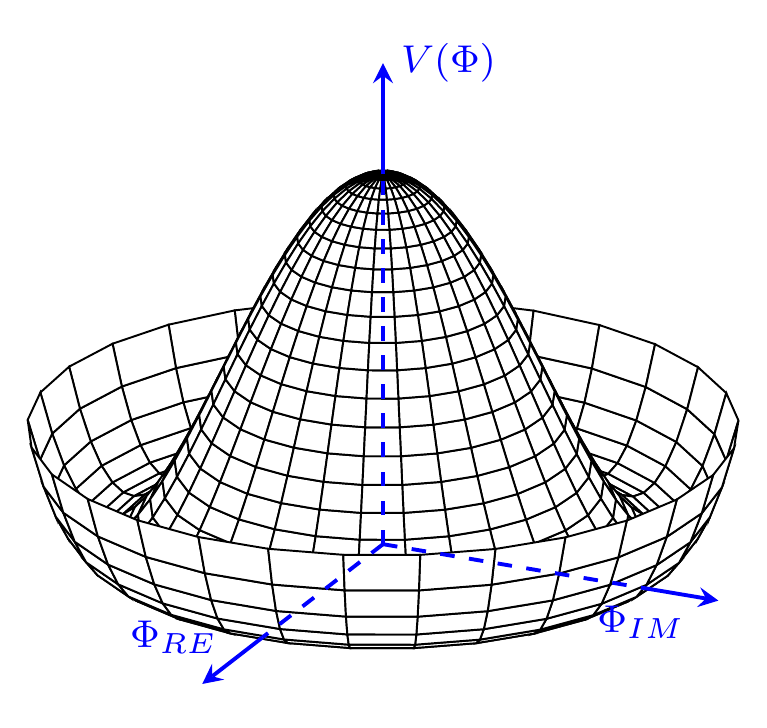
\begin{tikzpicture}[scale=1.75]
        \begin{axis}[
            hide axis,
            %axis lines=middle,
%            axis on top,
%            axis line style={blue,dashed,thick},
%            ymin=-2,ymax=2,
%            xmin=-2,xmax=2,
%            zmin=-2,zmax=2,
            samples=30,
            domain=0:360,
            y domain=0:1.25,clip=false
        ]
        \addplot3 [surf, shader=flat, draw=black, fill=white, z buffer=sort]
           ({sin(x)*y}, {cos(x)*y}, {(y^2-1)^2});
        \draw[blue,thick,dashed] (axis cs:0,0,0) -- (axis cs:1,0,0)
                    node[below,font=\footnotesize]{$\Phi_{\text{IM}}$};
        \draw[blue,thick,-stealth] (axis cs:1,0,0) -- (axis cs:1.3,0,0)
                    node[above,font=\footnotesize]{};
        \draw[blue,thick,dashed] (axis cs:0,0,0) -- (axis cs:0,-1,0)
                    node[left=2mm,font=\footnotesize]{$\Phi_{\text{RE}}$};
        \draw[blue,thick,-stealth] (axis cs:0,-1,0) -- (axis cs:0,-1.5,0)
                    node[right=1mm,font=\footnotesize]{};
        \draw[blue,thick,dashed] (axis cs:0,0,0) -- (axis cs:0,0,1)
                    %node[left=2mm,font=\footnotesize]{$\phi_{\text{RE}}$}
                    ;
        \draw[blue,thick,-stealth] (axis cs:0,0,1) -- (axis cs:0,0,1.3)
                    node[right,font=\footnotesize]{$V(\Phi)$};
        \end{axis}
    \end{tikzpicture}
    \caption{Higgs potential $V(\Phi^\dagger \Phi)$ for $\mu^2<0$ and $\lambda>0$ also called the mexican hat potential.}
    \label{hat}
\end{figure}

Electroweak symmetry breaking refers to the choice of ground state
\begin{align}\label{vmin}
	\Phi_0=\frac{1}{\sqrt{2}}\left(\begin{array}{c}
		0 \\
		v
	\end{array} \right)
	% \Phi =\sqrt{-\frac{\mu^2}{2\lambda}}=\frac{v}{\sqrt{2}}  \qquad \lambda >0
\end{align}
where $v=-\frac{\mu^2}{\sqrt{2}}$  is called the vacuum expectation value.\\


%Now, since the potential depends on $\Phi^\dagger \Phi$, We can select  $\Phi$ in the form 
%\begin{align}\label{doublet}
 %\Phi=\frac{1}{\sqrt{2}}\left(\begin{array}{c}
%0 \\
%v+h
%\end{array} \right) %\equiv v
%\end{align}
%here $\phi^+=0$ and h is a Higgs field  with respect to the minimal value v.

%Due to the conservation of electric charge,  only a neutral scalar field can acquire a vacuum expectation value.
%With this choice the scalar doublet has U (1)Y charge (hypercharge) $Y_\Phi$= 1
%and the electromagnetic charge is 
%\begin{align}
 %   Q=\frac{1}{2}(\sigma_3+Y)
%\end{align}
%so Q($\phi$) = 0. That is, electromagnetism is unbroken by the scalar VEV. The equation \ref{doublet} breaks the symmetry
%\begin{align}
%SU(2)_L  \otimes U(1)_Y \rightarrow U(1)_{em}
%\end{align}
Taking \ref{vmin} and substituting in $\mathcal{L}_\text{Higgs}$, we get 
\begin{align}\label{W}
\begin{split}
%(D_\mu \Phi)^\dagger (D^\mu \Phi) &=\left| \left(\partial_\mu+(ig/2)\sigma^iW^i_\mu+i\frac{1}{2} g' B_\mu \right)\frac{1}{\sqrt{2}}\left(\begin{array}{c}
%0 \\
%v
%\end{array} \right) \right|^2 \notag\\
%&=\frac{v^2}{8}\left| \left(g\sigma^i W^i_\mu + g' B_\mu \right) \left(\begin{array}{c}
%0 \\
%1
%\end{array} \right)        \right|^2 \notag\\
%&=\frac{v^2}{8}\left(\begin{array}{c}
 %    gW^1_\mu-igW^2_\mu \\
  %    -gW^3_\mu+g'B_\mu
%\end{array} \right) \notag\\
(D_\mu \Phi)^\dagger (D^\mu \Phi)& =\frac{v^2}{8} \left(g^2 ((W^1_\mu)^2 +(W^2_\mu)^2 )+( gW^3_\mu -g'B_\mu)^2 \right)
\end{split}
\end{align}

we define the physical vector boson $W^-_\mu$. $W^+_\mu$ and $Z$ 
\begin{align} 
W^{\pm}_\mu=\frac{1}{\sqrt{2}} (W^1_\mu \mp iW^2_\mu) \label{smo}\\ 
Z_\mu=\frac{1}{\sqrt{g^2+g'^2}}\left(gW^3_\mu -g'B_\mu   \right) \label{zboson}
\end{align}

%From equation \ref{smo}, we can express $W^1_\mu$ and $W^2_\mu$ in terms of $W^{+}_\mu$ and $W^{-}_\mu$
%\begin{align}\label{s2}
%W^{1}_\mu=\frac{W^{+}_\mu+W^{-}_\mu}{\sqrt{2}} \qquad  W^{2}_\mu=i\frac{W^{+}_\mu - W^{-}_\mu}{\sqrt{2}}
%\end{align}

%and the mass term
%\begin{align}   
 %    \frac{v^2}{8}g^2 W^\dagger_\mu W^\mu \rightarrow \frac{1}{2} \left( \frac{g v}{2} \right)^2      \notag
%\end{align}
Now introducing \ref{smo} and \ref{zboson} in \ref{W},
\begin{align}
(D_\mu \Phi)^\dagger (D^\mu \Phi)=\frac{v^2}{8}\left(2g^2 W_\mu^+ W^{\mu-} + (g^2+g'^2)Z_\mu Z^\mu  \right)  
\end{align}
from the coeficients, we get the $W$ and $Z$ mass  
\begin{align}
m_W=\frac{gv}{2} \qquad  m_Z=\frac{v}{2}\sqrt{g^2+g'^2}
\end{align}

%and the photon that in this case is the field A
%\begin{align}
 %       A_\mu=\frac{1}{\sqrt{g^2+g'^2}}\left(g'W^3_\mu +gB_\mu   \right)
%\end{align}
%with mass 
%\begin{align}
 %       m_A=0
%\end{align}

The last part of the lagrangian is the Yukawa lagrangian
\begin{align}
\mathcal{L}_\text{yukawa}=\sum_{m,n}^{3}  \Gamma^u_{mn}\bar{q}_{m\text{,}L} \tilde{\Phi} u_{n\text{,}R}+\Gamma^d_{mn}\bar{q}_{m\text{,}L} \Phi d_{n\text{,}R}+\Gamma^e_{mn}\bar{l}_{m\text{,}L} \Phi e_{n\text{,}R}+h.c
\end{align}
The matrices $\Gamma_{mn}$ describe the so called Yukawa couplings between Higgs doublet $\Phi$ and the fermions.\footnote{Here $
	\tilde{\Phi}=i\sigma^2 \Phi^\dagger =\left(\begin{array}{c}
	\phi^{0^\dagger} \\
	-\phi^-
	\end{array} \right)
	% \Phi =\sqrt{-\frac{\mu^2}{2\lambda}}=\frac{v}{\sqrt{2}}  \qquad \lambda >0
	$ is necessary for the correct transformation in the case of up quarks. \\
h.c refers to hermitian conjugate terms.  }  The indices  m and n mean sum over the families. \\
%It is required to have two representations of Higgs fields
%with $Y=\frac{1}{2}$  and $\frac{1}{2}$ to give masses to  quarks and electrons.
  

By using \ref{vmin} it on $\mathcal{L}_\text{yukawa}$,  it is obtained for $u$ quark
\begin{align*}
\frac{\Gamma^u_{uu}v}{\sqrt{2}}(\bar{u_L}u_R+\bar{u_R}u_L)
\end{align*}
from which the masses for the fermions shown to be proportional to the Yukawa couplings
\begin{align*}
m_u=-\frac{\Gamma^u_{uu}v}{\sqrt{2}}
\end{align*}
 
\pagebreak



\section{Higgs production mechanisms}
During a particle collision, there are various ways that the Higgs boson can be created. The most common is the gluon gluon fusion process ($gg$F) which is the process which involve two gluons  mediated by the exchange of a virtual, heavy top
quarks.  Another process  is vector boson fusion (VBF), where two fermions interact via a vector boson ($W$ or $Z$ ) and create a Higgs along with other particles. There is also the vector higgs process (VH), where the creation of particles using vector boson comes from a interaction between fermions and anti fermions\cite{pd}. These processes are shown in the figure \ref{psu} \\

In the recent years, people have studied the top anti top Higgs  ($t\bar{t}H$) process, in order to detect a Higgs boson, via multilepton signals\cite{th1}.
In this process, the creation of a Higgs boson comes from a intection via $t\bar{t}$. In the figure \ref{psu}, the $t\bar{t}H$ starts with 2 gluons which decay to two $t\bar{t}$ pairs and after that , the interaction $t\bar{t}$  generates a Higgs. The last process, subject of study in this thesis, is the top Higgs ($tH$) process. This process is a rare expected process with a very small production rate\cite{pd}.  In the figure \ref{thw}, is another way to produce $tH$, in association with a $W$.

\begin{figure}[htbp]
\centering
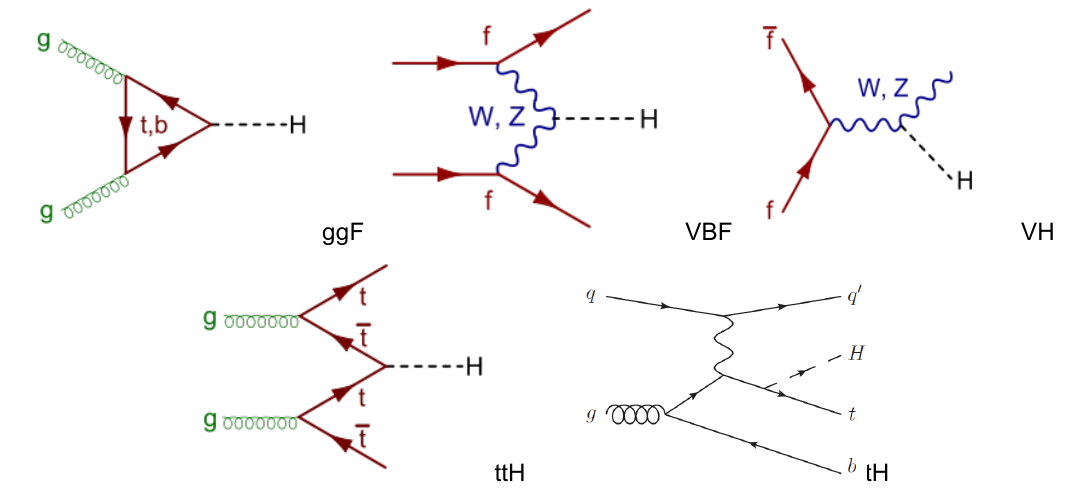
\includegraphics[scale=0.5]{Chapter1/pg.png}
\caption{Different Higgs production mechanism, from the most likely to least likely}
\label{psu}
\end{figure}


\begin{figure}[htbp]
\centering
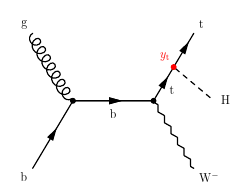
\includegraphics[scale=0.7]{Chapter1/thw.png}
\caption{$tHW$ mechanism}
\label{thw}
\end{figure}

In tH process, Higgs boson is radiated from a single top quark as shown in \ref{psu}. tH process is a new field of study, given that there are few experiments and its production rate (probability) is small, so the detection of Higgs bosons in this channel opens to new discoveries.
\\

In particle physics, cross section ($\sigma$) describes the likelihood of two particles interacting under certain conditions.
 Cross sections are expressed in barns , where 1 barn=$10^{-34}$ cm$^{2}$ .
\\
The cross section is important in the evaluation of events for specific processes. In order to get the number of events for a specific process,  the reaction rate $N$ is determined by the total cross section $\sigma$ and the luminosity L.\\
%L is called luminosity, that is the number of particle interactions can be produced in a detector per second . 
The unit of measurement of luminosity is  cm$^{-2}$s$^{-1}$.  Therefore, The reaction rate is 

\begin{align} \label{nr}
N_R=\sigma \text{L}
\end{align}
In practice, the luminosity is measured by counting the number of events for a well known process.

\begin{table}[ht]
\centering
\caption{	Higgs boson production cross sections  in pp collisions for $\sqrt{s}=13$TeV  (in pico barn) and number of events for an integrated luminosity of 35.9 fb$^{-1}$ for Run 2 \protect \cite{pd}}
\begin{tabular}{|c|c|c|}
\hline
Production mechanism &
$\sigma$ (picobarns pb) & Number of events \\
\hline
$gg$F & 48.93 & 1756587\\
\hline
VBF & 3.78 & 135702\\
\hline
$WH$ & 1.35 & 48465\\
\hline
$ZH$ &0.88 & 31592\\
\hline
$t\bar{t}$H & 0.50 & 18255\\
\hline
$tH$	& 0.015 & 560.39\\
\hline
\end{tabular}
\label{crt}
\end{table}

In the table \ref{crt} shows the Higgs production cross section for pp collision and the number of events produced using a integrated luminosity of $35.9 fb^{-1}$ , that is the luminosity measured for the Run 2 from LHC on 2016\cite{pd}.

\begin{figure}
\centering
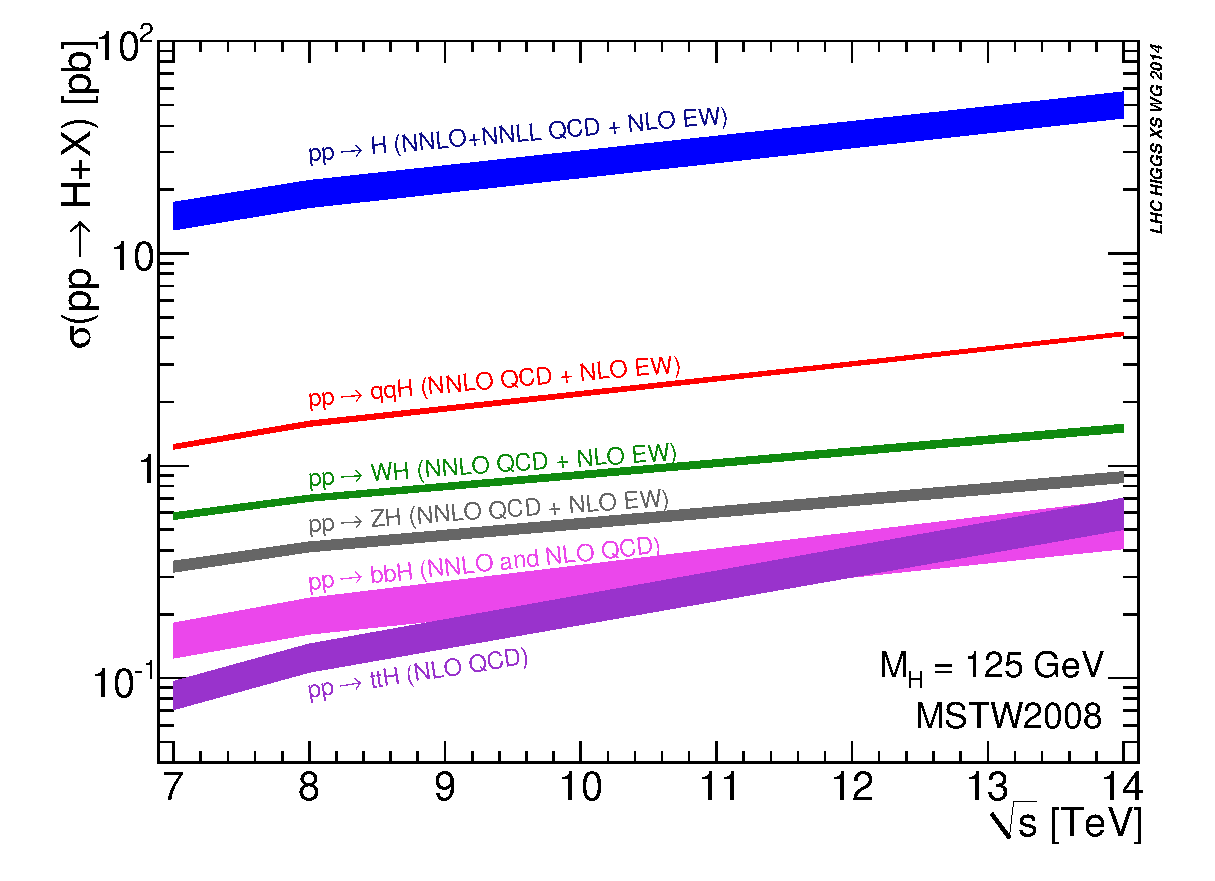
\includegraphics[width=12cm,height=7cm]{Chapter1/7-14xsec.eps}
\caption{
Cross section for different processes generated in a pp collision \protect \footnotemark }
 \label{csp}
\end{figure}

Here we can see ggF process have the biggest cross section of all Higgs mechanism and generates the greatest number of events possibles. For the processes tH and $t\bar{t}$H, they have the smallest cross section, so the probability for the processes is low and generates a small number of events. 
\pagebreak
\footnotetext{Taken from \url{ https://twiki.cern.ch/twiki/bin/view/LHCPhysics/LHCHXSWGCrossSectionsFigures}}
\section{Higgs decay rates}
In particle physics,two importatns properties are the lifetime and the decay rates of a particle. The lifetime is related to the total decay rate $\Gamma$, that is the probability per unit of time a particle decay, 
\begin{align}
    dN=-\Gamma N dt
\end{align}
with N the original number of particles before the decay. From here is evident that number of particles left in a decay is 

\begin{align}
N(t)=N_0 e^{-\Gamma t}
\end{align}

%For a particle that decays into several particle , $\Gamma$ is given by
%\begin{align}\label{dm}
%\Gamma=\frac{S}{2\hbar m_n}\int \left| M \right|^2 (2\pi)^4 \delta^4(p_1-p_2-...p_n)\times \prod_{j=2}^n 2\pi \delta (p_j^2-m_j^2 c^2)\theta (p_j^0)\frac{d^4 p_j}{(2\pi)^4}
%\end{align}
%where $m_n$ and $p_n$ are the mass and momentum of the particle n with n=1,2,3,... . S is a statistical factor that avoid identical particles counting. If there are no identical particles, S=1 ,and for identical particles $S=\frac{1}{s!}$ with s is the number of identical particles. $\mathcal{M}$ is the amplitude which is a momenta function that is calculated acording to the Feynman diagrams.$\theta(p_j^0)$ is a Heaviside function,
%$p_j$ is the outgoing momentum and $p^0_j=E_j/c>0$.\cite{griff}

The number of particles decreases over time exponentially and this can be measured. With this, it is possible determinate the mean lifetime\cite{griff}
\begin{align}
\tau=\frac{1}{\Gamma}
\end{align}
In case of  the decay rate to a specific process, it is necessary get the branching fraction of the process. 
The branching ratio for a decay process is the ratio of the number of particles which decay via a specific decay mode with respect to the total number of particles which decay via all decay modes.
\begin{align}
BR_i =\frac{\Gamma_i}{\sum_{i}\Gamma_i}
\end{align}
Where $\Gamma=\sum_i\Gamma_i$ is the total decay width (sum of all partial widths) of the particle and is related to lifetime of the particle: $\Gamma=1/\tau$.
Since the dimension of $\Gamma$ is the inverse of time, in our system of natural units, it is measured in inverse seconds,it has the same dimension as mass (or energy)\footnote{Cleaves H.J. (2011) Branching Ratio. In: Gargaud M. et al. (eds) Encyclopedia of Astrobiology. Springer, Berlin, Heidelberg} . The lifetime of the Higgs boson is predicted to be 1.56 $\times$ $10^{-22}$ seconds and corresponds to $\Gamma_H$ is about 4 MeV , but has not yet been measured due to the detector resolution\cite{cms-manual}.
\\
\begin{table}[!htbp] 
\caption{SM Higgs boson branching ratios for  $M_H$ =125 GeV \protect \cite{pd}}
\centering
\begin{tabular}{|c|c|}
\hline
Higgs decay & Branching ratio (BR)\\
\hline
$H \rightarrow$ b$\bar{b}$ &$58.4\%$ \\
\hline
 $H \rightarrow$ $W^+W^-$ &$21.4\%$ \\
\hline
$H \rightarrow$ $\tau^+ \tau^-$ & $6.27\%$\\
\hline
$H \rightarrow$ ZZ &$2.62\%$\\
\hline
$H \rightarrow$ $\gamma\gamma$ &$0.227\%$\\
\hline
$H \rightarrow$ Z$\gamma$ &$0.153\%$\\
\hline
$H \rightarrow$ $\mu^+\mu^-$ &$0.0218\%$\\
\hline
\end{tabular}
\label{higgs1}
\end{table}
The decay  $H \rightarrow$ $b\bar{b}$ have a branching ratio a bit more than 50$\%$, therefore is the most likely decay Higgs boson can decay. Due to this,  $H\rightarrow b\bar{b}$ is a very studied process and most likely to detect a Higgs boson in the data after reconstruction. The decay  $H \rightarrow$ $\mu^+\mu^-$ has a very low branching ratio. This decay is very rare but not imposible to detect in the future.  In this work the majority of the Higgs decays detected are from $WW$, $ZZ$, $\tau \tau$\\

\section{$tH$ production mechanism}
The production of $tH$, where a Higgs boson can be radiated
either from the top quark or from the exchanged $W$ boson in the two dominant leading order
diagrams in figure \ref{newth} provides a unique opportunity to study the relative sign of the coupling.
In SM , the two diagrams interfere negatively and thereby suppress the production cross section.
Any deviation from the SM can lead to a large enhancement of the event rate.
 $\kappa_t$ and $\kappa_V$ are the coupling parameters, where $\kappa_t$ is for the top and $\kappa_V$ for $W$ boson. \\

\begin{figure}[ht]
	\centering
	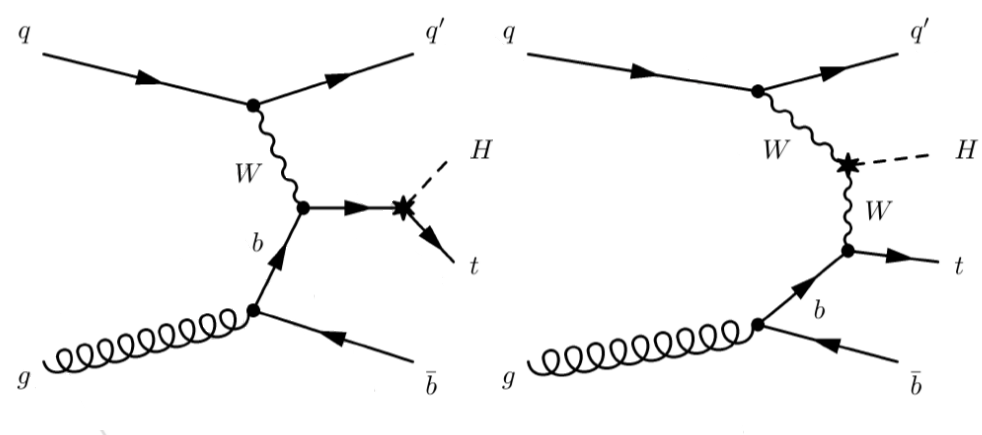
\includegraphics[scale=0.5]{Chapter1/newtHq.png}
	\caption{tH mechanism. Higgs radiated from a top quark (left). Higgs radiated from a W boson (right) \protect \cite{bb}} \label{newth}
\end{figure}
\pagebreak



\end{chapter}













